%! Author = sbbfti
%! Date = 10/06/2020


\section{Results}\label{sec:results}

The sensible heat losses from the skin to the environment are proportional to the difference between the \ac{t-sk} and \ac{t-op}, as shown in Equation~\ref{eq:c-r}.
Consequently, for values of \ac{t-op} higher than \ac{t-sk} the body start gaining sensible heat from its environment and the term \ac{c-r} becomes negative.
Figure~\ref{fig:comparison_models}A shows how the sensible heat losses estimated with the \mycite{GaggeSET} and the \mycite{Jay2015} models vary as a function of \ac{t-op}, \ac{rh}, and \ac{v}.
The former model iteratively determines \ac{t-sk}, while the latter assumes it to be constant and equal to 35~$^{\circ}$C.
This explains the difference in \ac{c-r} determined by the two models.
For \ac{t-op} higher than those at which \ac{w-max} occurs (Figure~\ref{fig:comparison_models}B), our model estimates that heat energy gets stored in the body and consequently \ac{t-sk} increases, as shown in Figure~\ref{fig:results_model_2}C\@.
This reduces the rate at which sensible heat gains increase.
The values of \ac{w} and the respective values of \ac{w-max} for two air speeds are shown in Figure~\ref{fig:comparison_models}B\@.
It can be observed that the critical operative temperature at which \ac{w} equals \ac{w-max} is a inversely proportional to the value of \ac{rh}.

\begin{figure}[thb!]
    \centering
    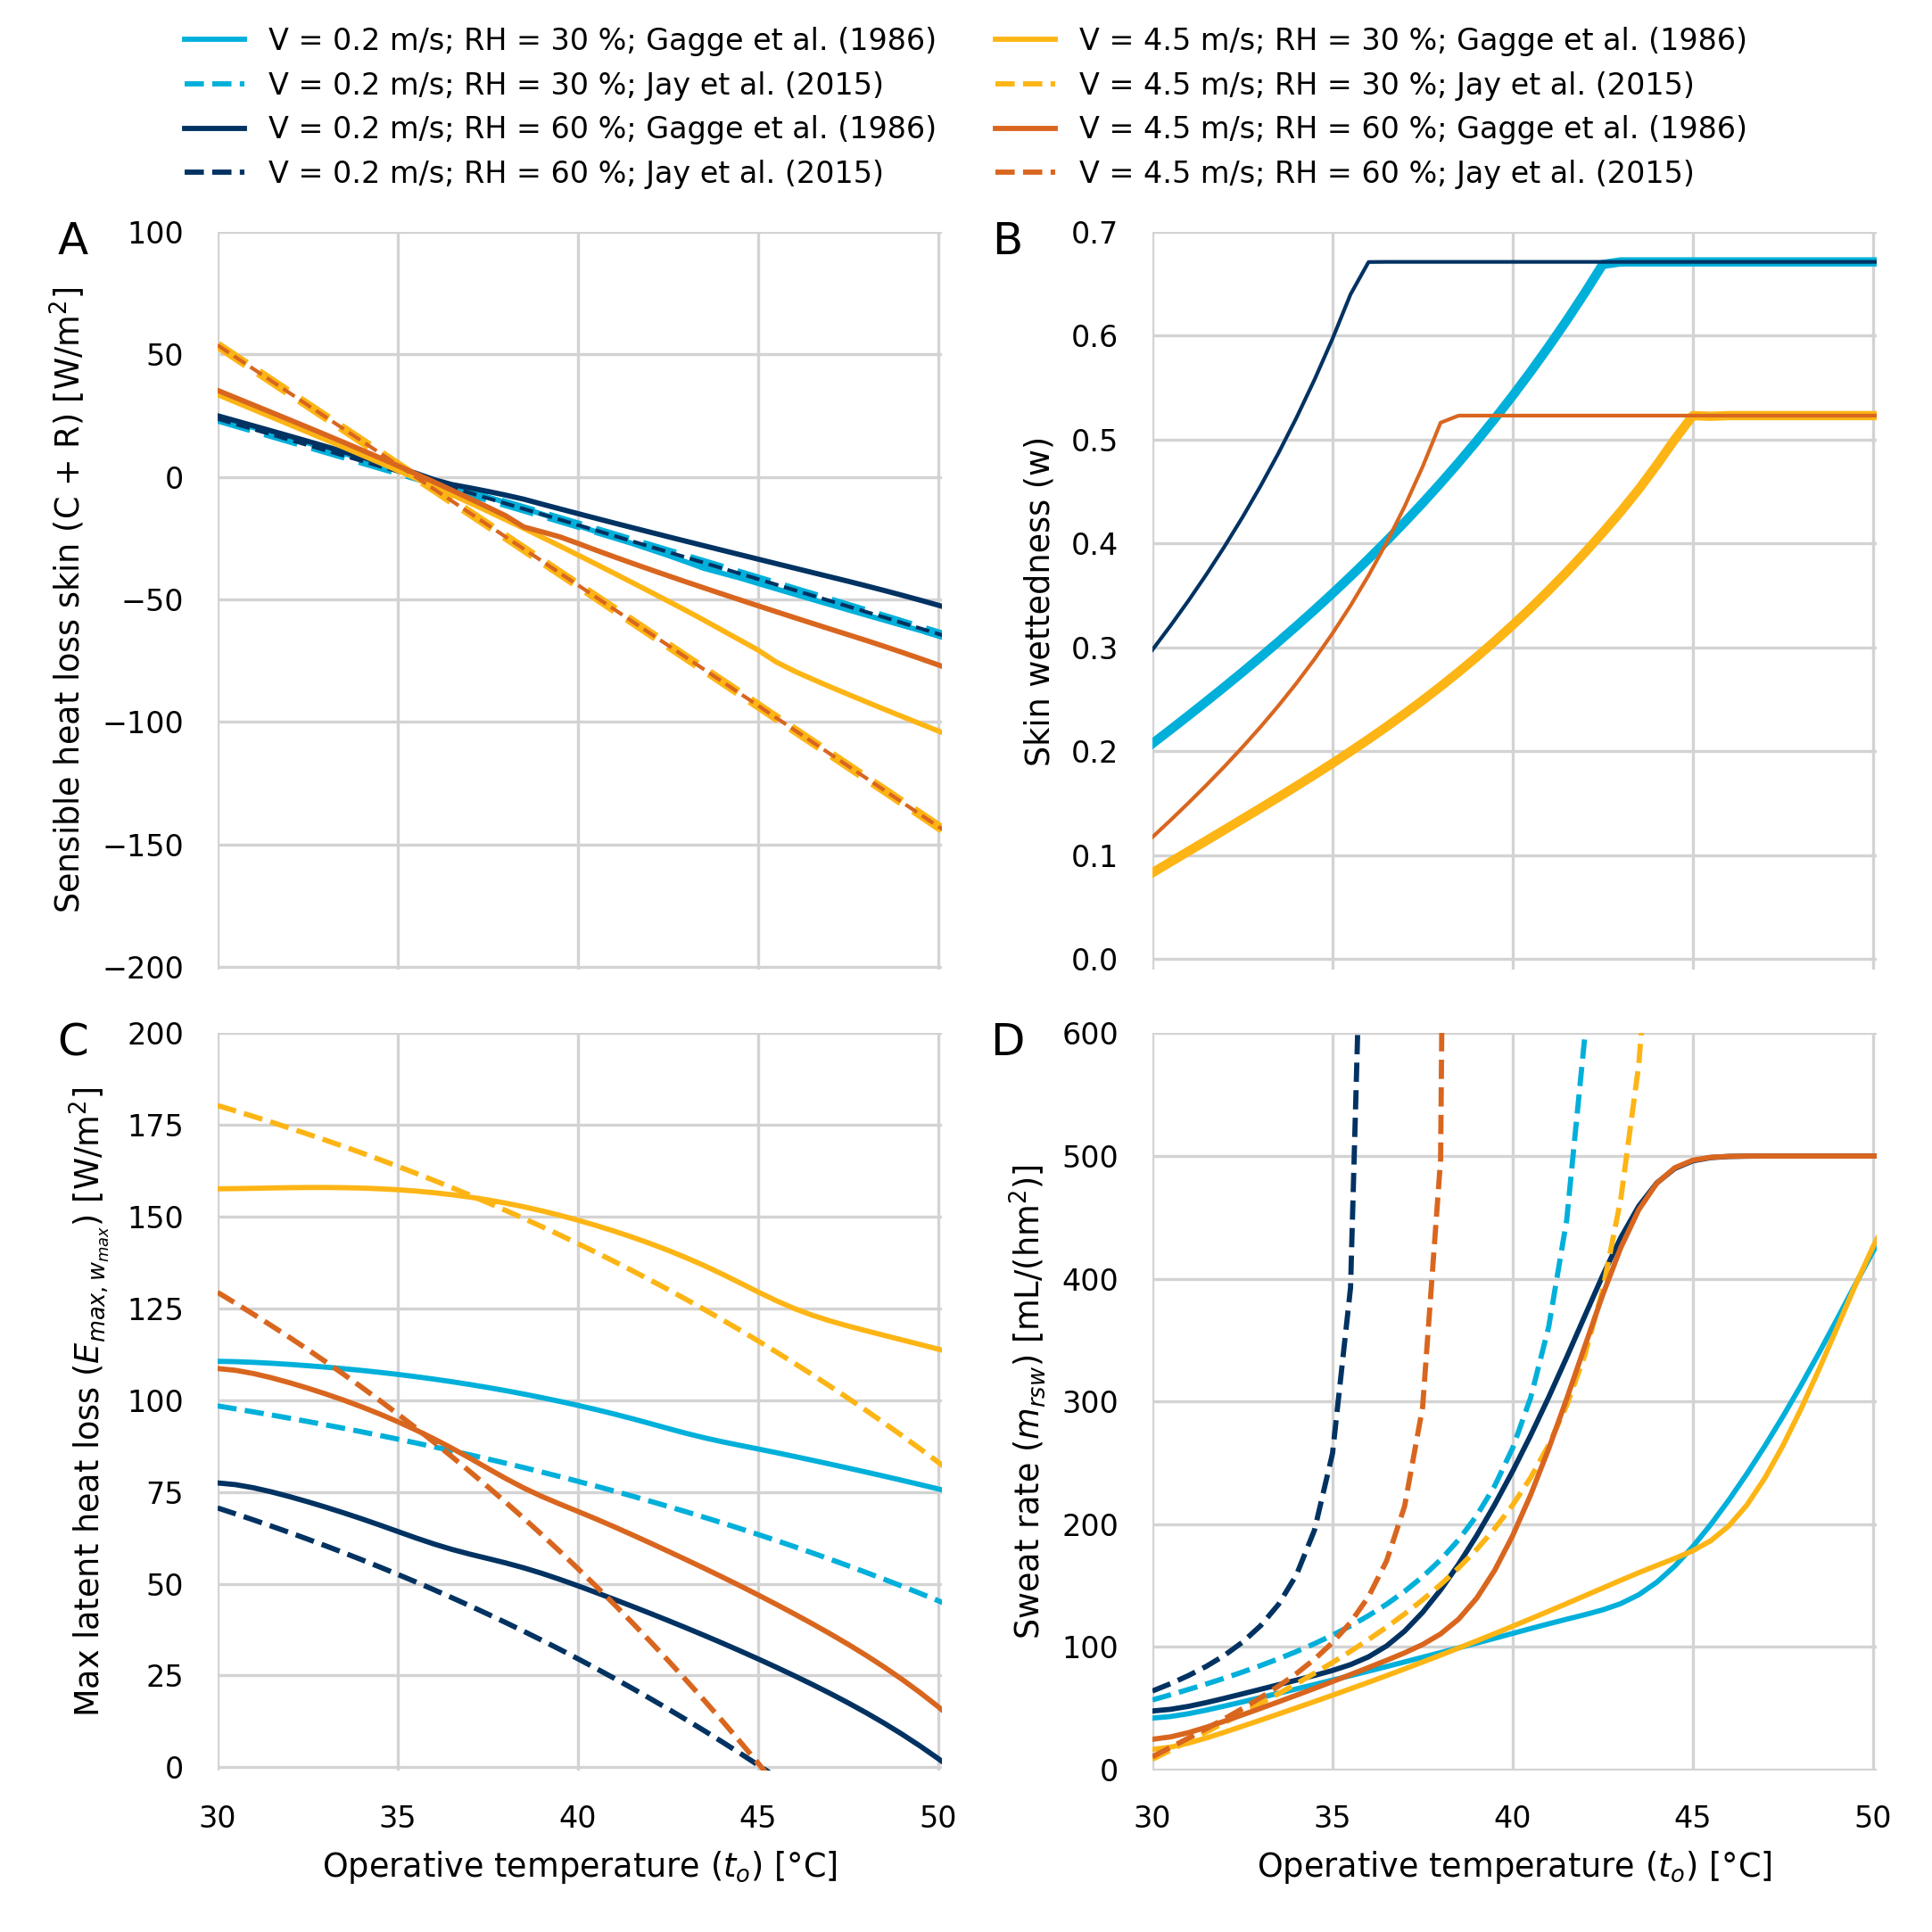
\includegraphics[width=\textwidth]{figures/comparison_models_v2.png}
    \caption{Shows how the results obtained with the the energy models proposed by \mycite{Jay2015} and \mycite{GaggeSET} vary as a function of the \ac{t-op}.
    Each Figure shows the results obtained using a combination of two values of \ac{rh} and \ac{v}.
    Figure A - sensible heat losses from the skin vary.
    Figure B - skin wettendess.
    Figure C - Maximum latent heat loss estimated using \ac{w} = \ac{w-max}.
    Figure D - Sweat rate.}
    \label{fig:comparison_models}
\end{figure}

The negative effect that an increase in \ac{v} has on the sensible heat gains is, however, compensated by a greater increase in the \acf{e-sk} that the body can dissipate towards the surrounding environment.
For example, when \ac{t-op}~=~45~$^{\circ}$C and \ac{rh}~=~30~\%, an increase in \ac{v} from 0.2 to 4.5~m/s increases the sensible heat gains (\acs{c-r}) by 29 W/m\textsuperscript{2} while increasing \ac{e-sk} by 45~W/m\textsuperscript{2}, hence, increasing \ac{v} has a net positive effect.
Figure~\ref{fig:comparison_models}C shows the values of \ac{e-max} estimated by replacing \ac{w} in Equation~\ref{eq:latent-skin} with \ac{w-max}.
The value of \ac{e-max} decreases as the \ac{t-op} increases since \ac{p-a} grows more rapidly than \ac{p-sk}.
For a set combination of \ac{v} and \ac{t-op} the value of \ac{e-max} decreases as the value of \ac{rh} increases since humid air has a higher \ac{p-a} than dry air.
The reduction in \ac{e-max} estimated by our model is lower than the one estimated by \mycite{Jay2015} since we do not assume \ac{t-sk} to be constant.

The value of \ac{m-sweat} is shown in Figure~\ref{fig:comparison_models}D\@.
The difference between the results obtained with the two heat balance models can be attributed to the fact that \citeauthor{Jay2015} calculate the value of \ac{m-sweat} as a function of the required latent energy that the body should in theory dissipate to achieve thermal neutrality.
Hence it comprises both regulatory sweating and water loss through skin diffusion.
On the other hand, \citeauthor{GaggeSET} calculate the value of \ac{m-sweat} as a function of regulatory signals and they assume that \ac{m-sweat} cannot exceed 500~mL/h, and it does not accounts for water loss through skin diffusion.
\citeauthor{GaggeSET} also do not account for water losses through skin diffusion.

\begin{figure}[thb!]
    \centering
    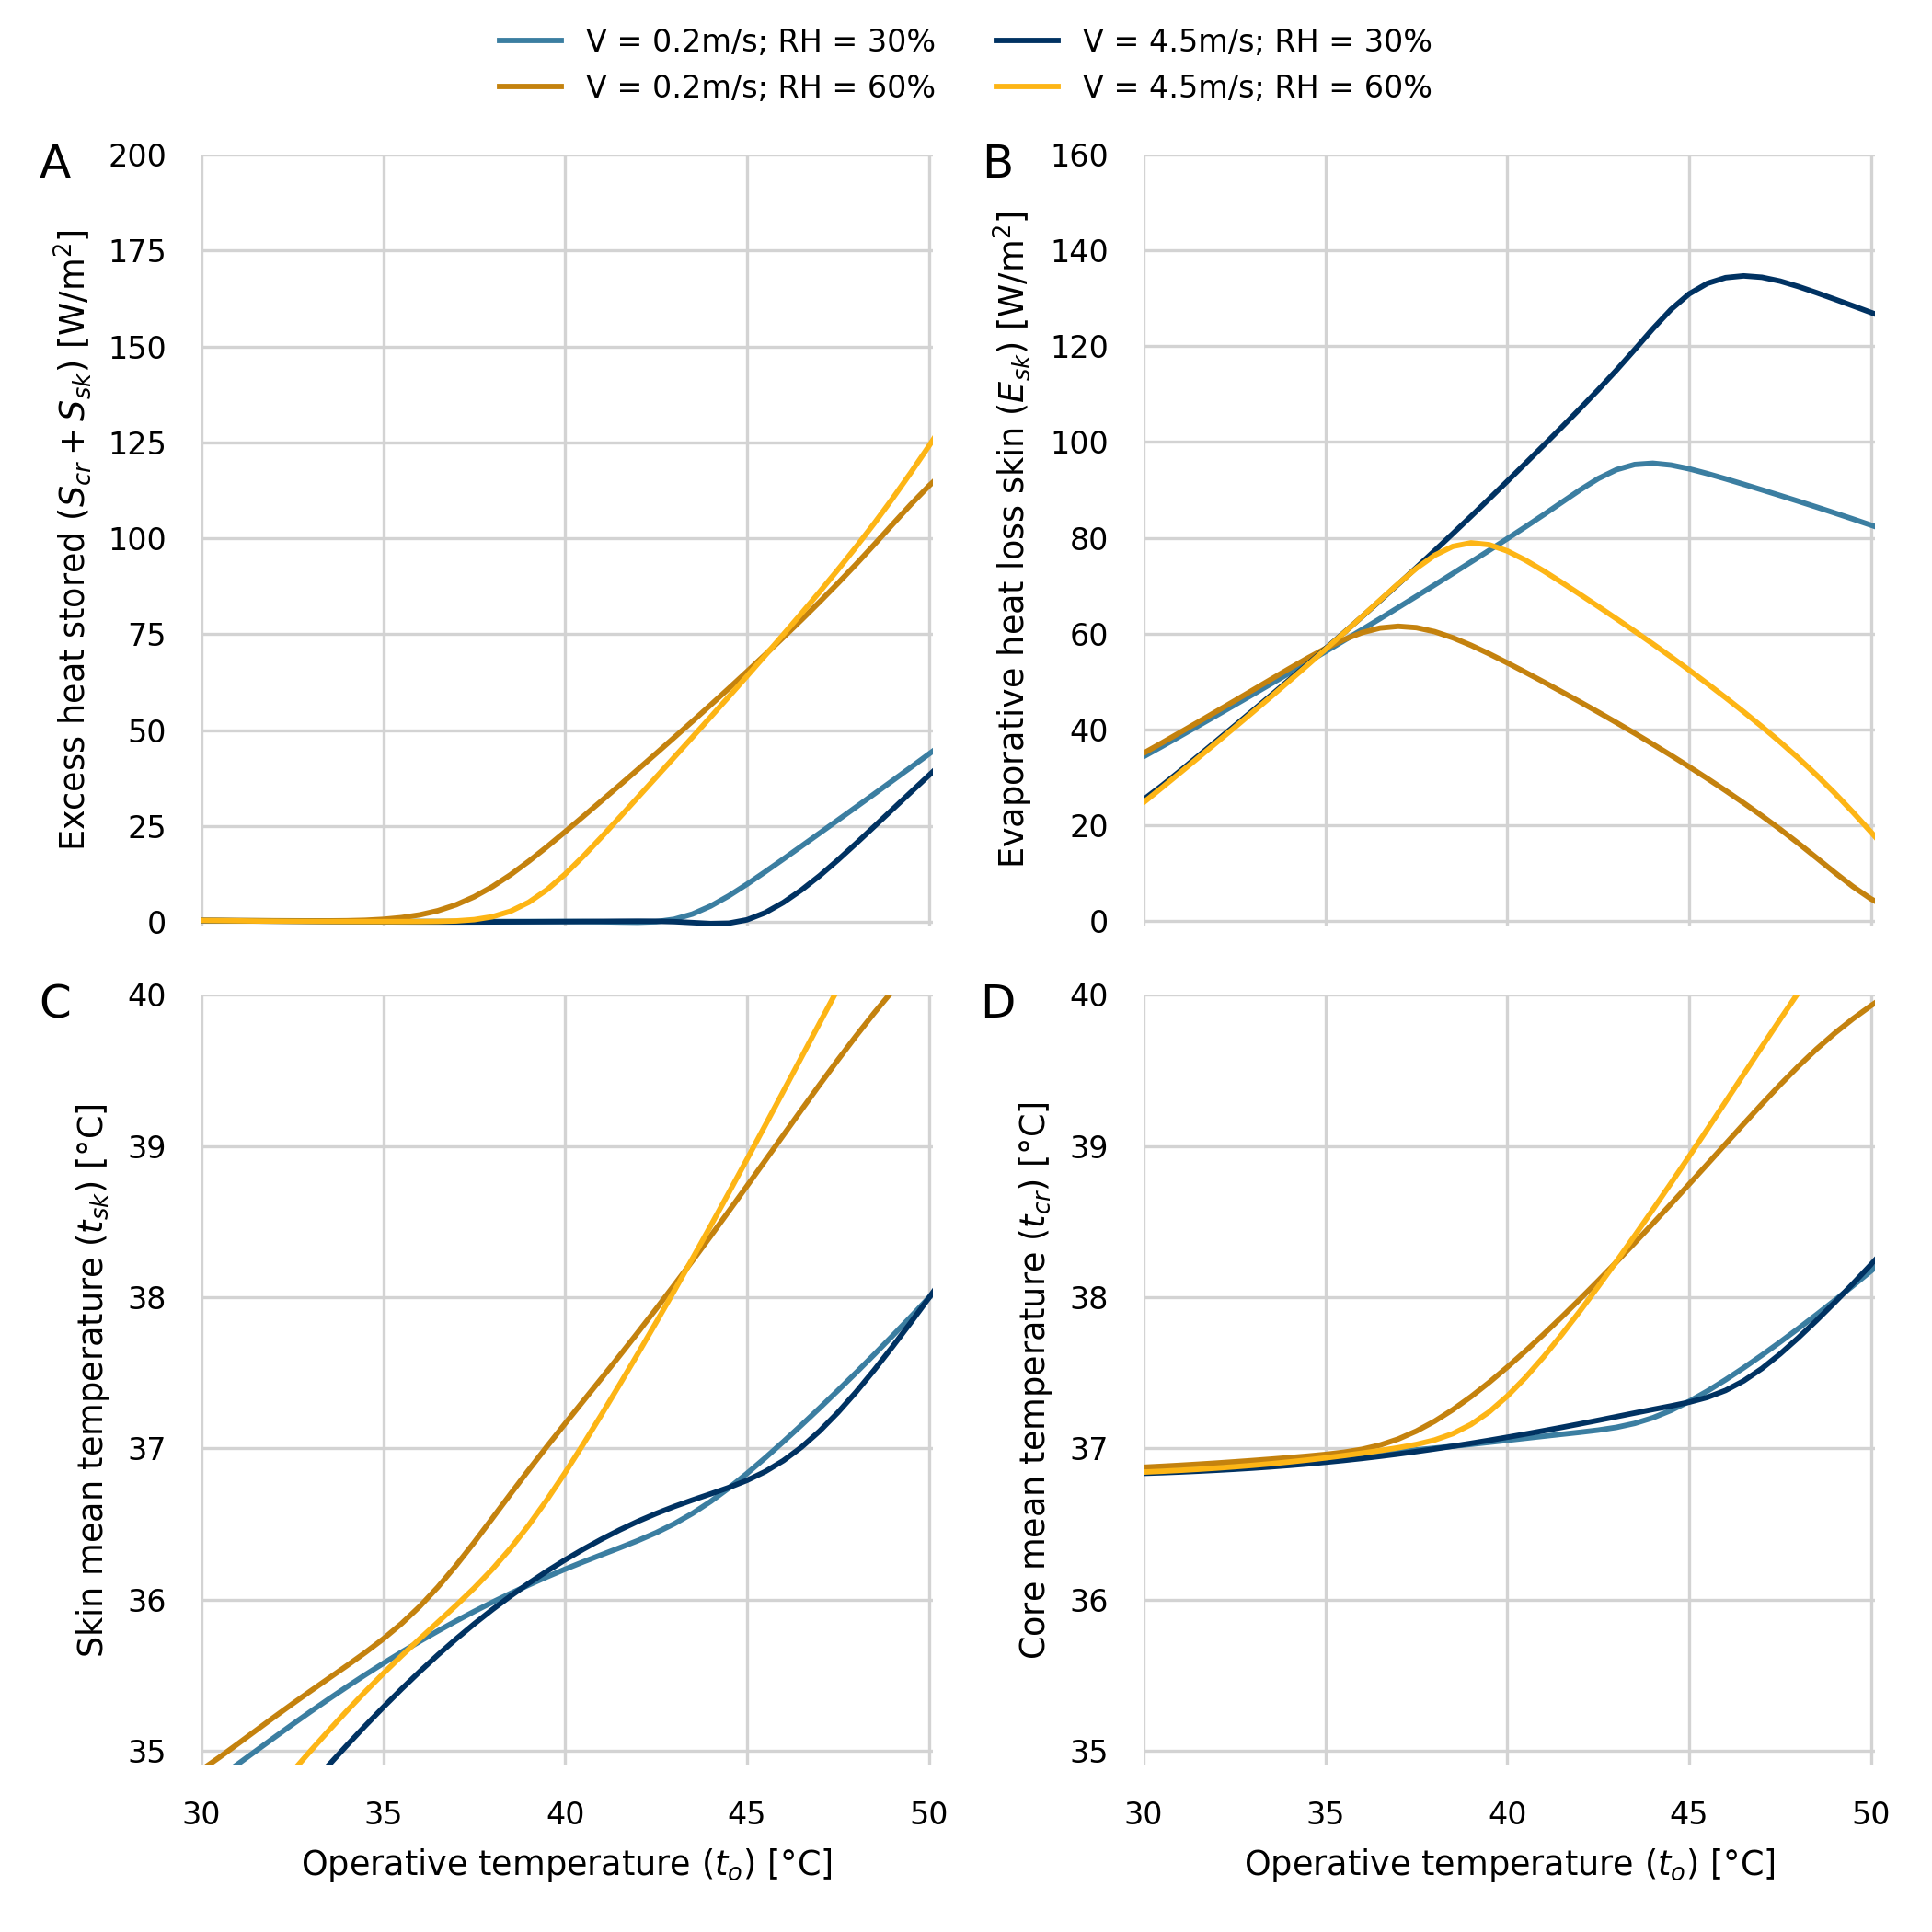
\includegraphics[width=\textwidth]{figures/results_model_2.png}
    \caption{Caption}
    \label{fig:results_model_2}
\end{figure}

The estimated values of excess heat stored in the human body, \ac{t-sk}, and \ac{t-cr} are shown in Figure~\ref{fig:results_model_2}A, ~\ref{fig:results_model_2}C, and ~\ref{fig:results_model_2}D, respectively.
As soon as the body cannot longer dissipate exogenous and endogenous heat gains, the excess heat gets stored in the human body and both \ac{t-sk} and \ac{t-cr} rise.
The \ac{t-op} at which \ac{t-cr} with elevated air speed exceeds the value of \ac{t-cr} for the `still air' condition is when the use of air movement becomes detrimental.
While, when the energy stored becomes greater than zero is the conditions which demarcates when heat strain would start to occur.

The combination of \ac{t-op}, \ac{rh}, and \ac{v} at which heat strain would start to occur since the body is no longer able to dissipate all the heat gains are presented in Figure~\ref{fig:comparison_air_speed}.
The Figure shows the results obtained with the \mycite{GaggeSET} and the \mycite{Jay2015} models.

\begin{figure}[thb!]
    \centering
    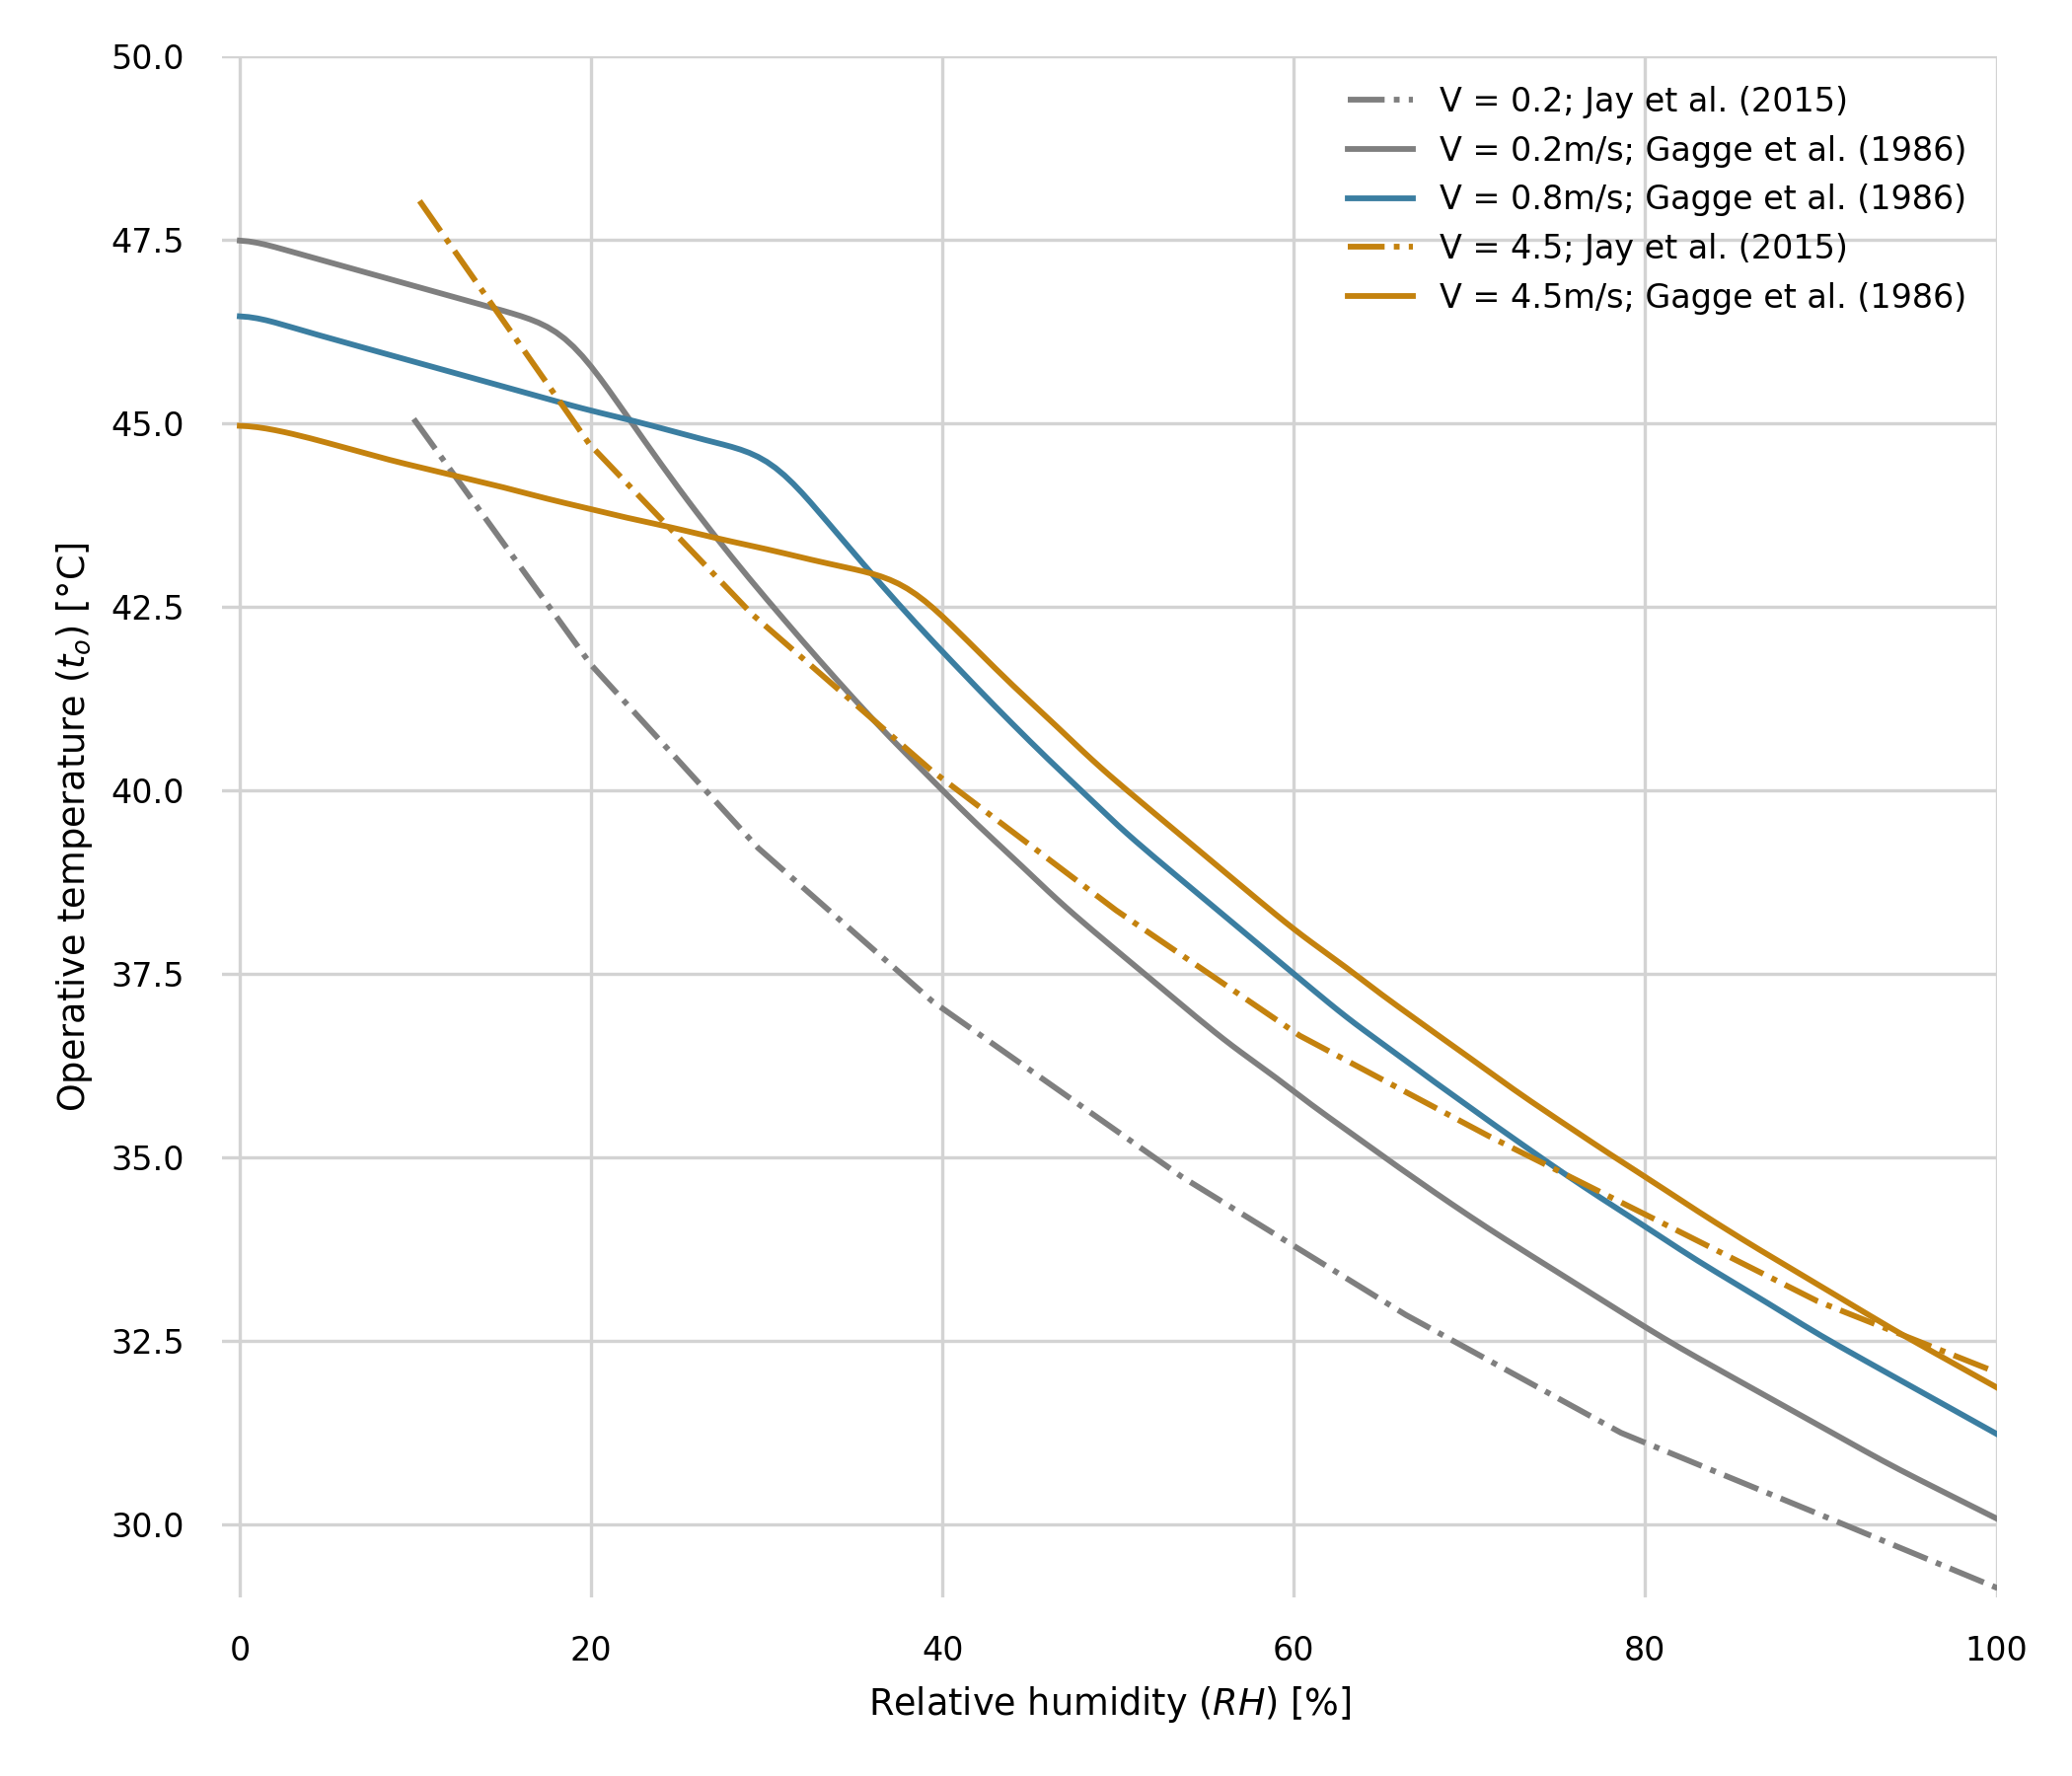
\includegraphics[width=\textwidth]{figures/comparison_air_speed.png}
    \caption{Compares the results between the SET model and Ollie's model.
    Each line demarcates point above which the body cannot longer dissipate all the endogenous and exogenous heat gains, hence the extra energy gets stored in the body and it causes the \acf{t-cr} to increase.}
    \label{fig:comparison_air_speed}
\end{figure}

It should be noted that the limit presented in Figure~\ref{fig:comparison_air_speed} is not the limit above which an increase in \ac{v} is no longer beneficial.
Each line demarcates the region in which thermal stress is estimated to occur and not all individuals would be able to compensate for endogenous and exogenous heat gains.
For a specific value of \ac{v}, the maximum \ac{t-op} at which cardiovascular strain is estimated to occur decreases as the value of \ac{rh} increases.
In addition, it can be observed that for a specific value of \ac{rh}, as the value of \ac{v} increases the overall increase in the maximum critical temperature rapidly decreases.
For example, in an environment with \ac{rh}~=~60~\%, increasing \ac{v} from 0.2~m/s to 0.8~m/s then to 4.5~m/s lead to an increase of the critical temperature of approximately 2.3~$^{\circ}$C and 0.8~$^{\circ}$C, respectively.

To better understand how personal factors would impact the body ability to dissipate heat gains we calculate when heat strain would occur for different combinations of \ac{met} and \ac{clo}.
Results for people wearing light summer clothing (walking shorts, short-sleeve shirt and sandals, \acs{clo} = 0.36 clo), and office summer clothing (trousers, short-sleeve shirt, and closed shoes \acs{clo} = 0.5 clo) who are either seated reading or writing (\ac{met} = 1.0 met) or standing relaxed (\ac{met} = 1.2 met) are shown in Figure~\ref{fig:met_clo}.
Results show that for \ac{v} = 0.2 m/s decreasing \ac{met} by 0.2 met is more beneficial than reducing \ac{clo} by 0.14.
On the other hand, when \ac{v} = 0.8 m/s both aforementioned interventions lead to similar results since latent heat loss can compensate for an increase in \ac{met} as long as the value of \ac{clo} remains low.

\begin{figure}[thb!]
    \centering
    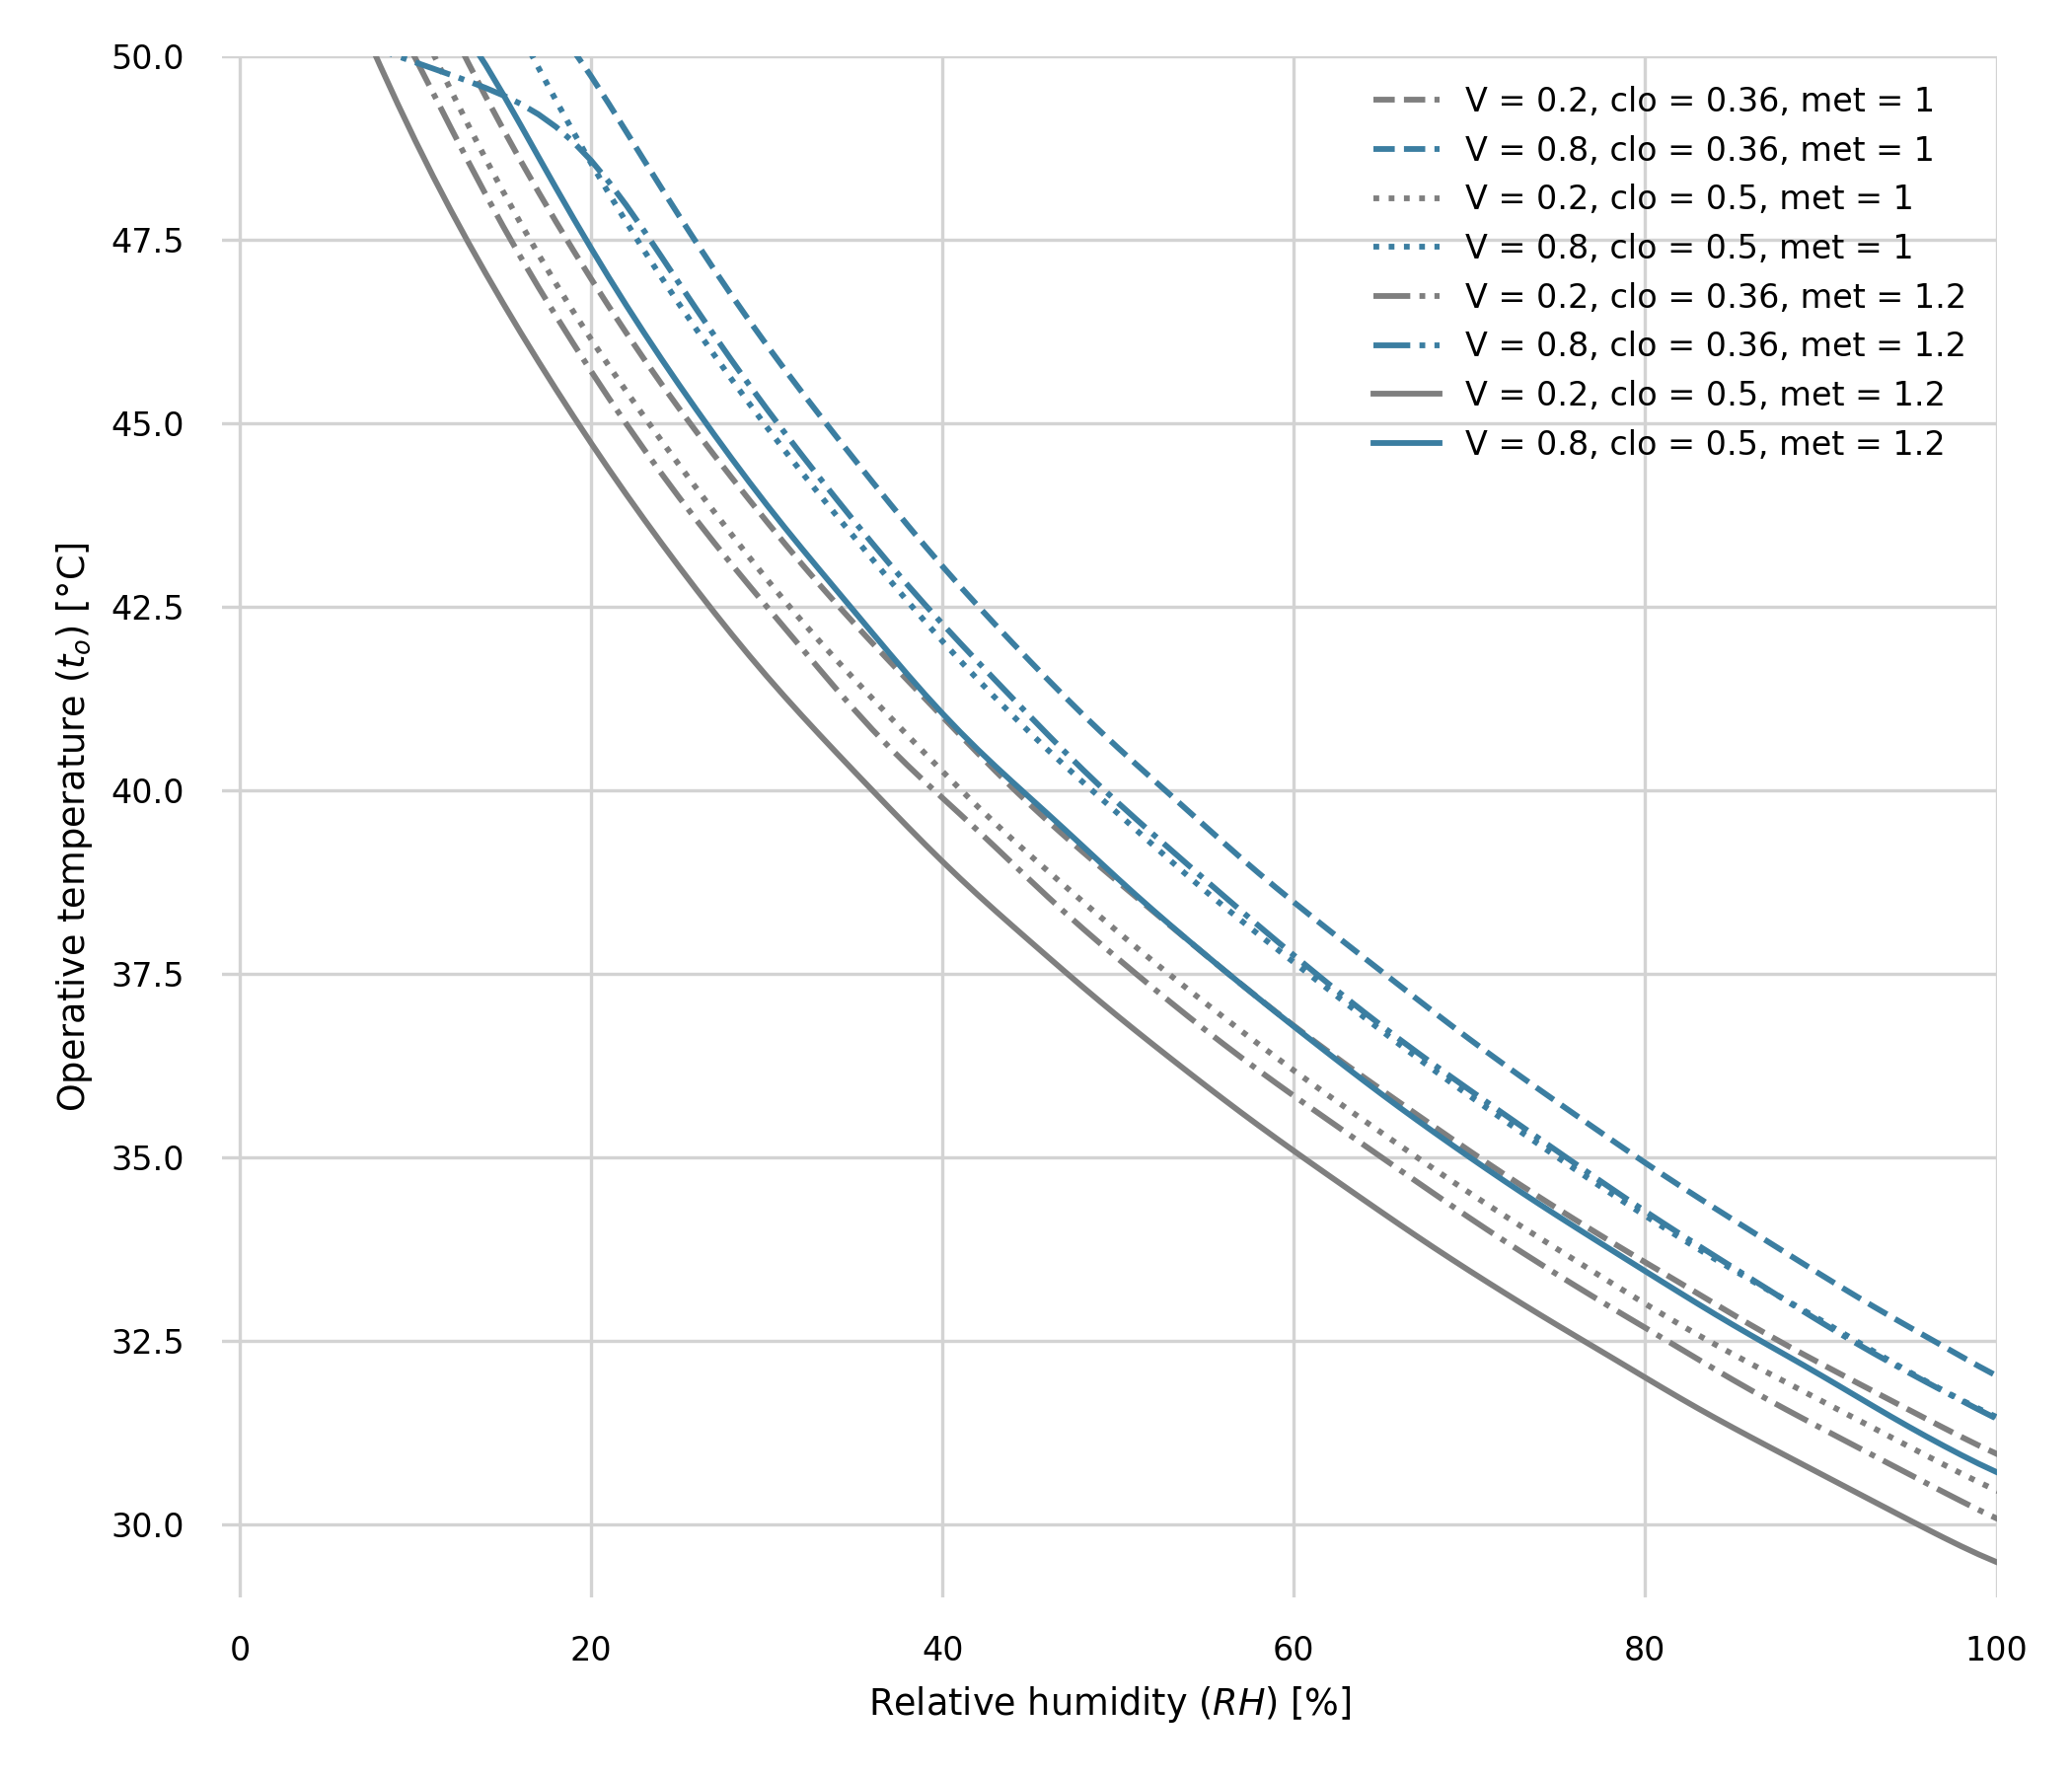
\includegraphics[width=\textwidth]{figures/met_clo.png}
    \caption{Each line demarcates how different combinations of personal factors (e.g., \ac{met}, \ac{clo}) and environmental factors affect the point above which the body cannot longer dissipate all the endogenous and exogenous heat gains}
    \label{fig:met_clo}
\end{figure}

The environmental conditions above which the use of elevated air speeds would actually be detrimental for the health of the people is shown in Figure~\ref{fig:energy_storage_delta}.
This Figure depicts the area in which electrical fans should not be used, and shows the lines above which thermal strain is expected to occur (as previously shown in Figure~\ref{fig:comparison_air_speed}).
We also plotted the maximum extreme weather conditions recorded worldwide over the las 10 years.
Each dot represents the most extreme dry-bulb temperature and the \ac{rh} value measured for each weather station.
From Figure~\ref{fig:energy_storage_delta} it can be observed the area in which electrical fans are dangerous for humans narrows as \ac{v} decreases and approaches 0.2~m/s.
In addition, for a specific value of \ac{rh}, as the value of \ac{v} increases the critical temperature at which thermal strain would occur also increases, however, at the same time the temperature above which fans should not be used also decreases by a greater amount.
Based on the climate data obtained from the 2017 ASHRAE Handbook--Fundamentals we estimated that in approximately 70~\% of the locations thermal strain should not occur even without air movement, however, this number increases to 86~\% and 93~\% when \ac{v} is increased to 0.8~m/s and 4.5~m/s, respectively.
The use of fans would still be beneficial in the great majority of the locations worldwide.
With the exception of only two locations where the use of \ac{v} higher than 0.8~m/s would be detrimental for the human body.

% https://advances.sciencemag.org/content/6/19/eaaw1838

% todo report estimated sweat heat lossess too, either using a table or a heatmap

\begin{figure}[thb!]
    \centering
    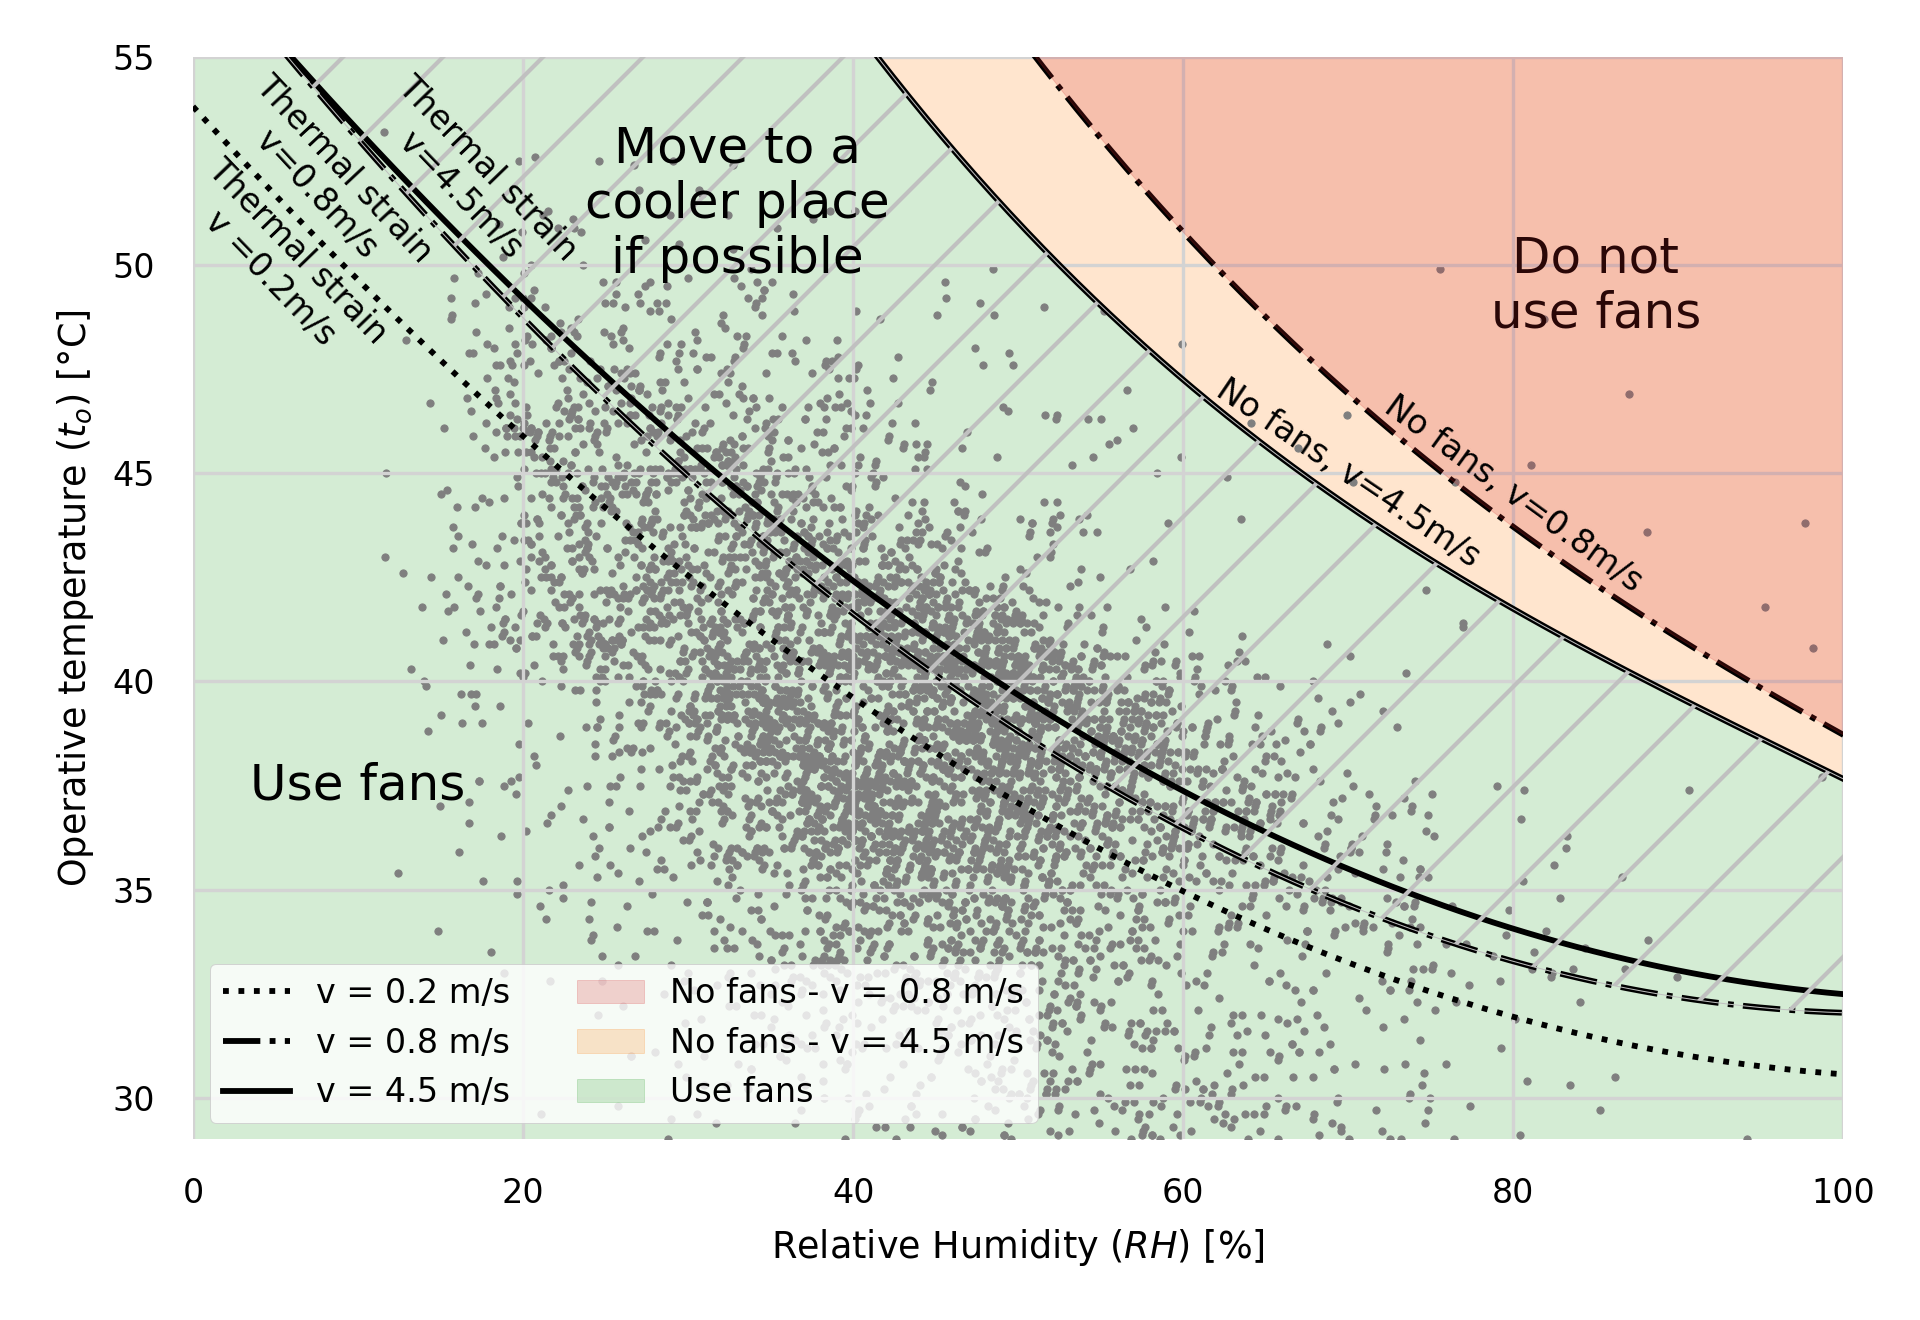
\includegraphics[width=\textwidth]{figures/use_fans.png}
    \caption{The green area shows the environmental conditions in which the use of fans is beneficial since they provide additional cooling to the human body.
    In the hatched area, while the use of fans it is still beneficial, people are most likely to suffer from heat stress.
    Finally the red area demarcates the region in which electrical fans should not be used.
    The dots show the maximum extreme climate conditions recorded over the last 10 years in more than 5000 locations worldwide.
     These results were calculated assuming \ac{t-r} = \ac{t-db}, \ac{clo} = 0.5~clo, \ac{met} = 1.0~met.}
    \label{fig:energy_storage_delta}
%    todo replace this figure with the core body delta
\end{figure}


